\documentclass[../main.tex]{subfiles}

\begin{document}

    El gran poder expresivo con el que cuentan los lenguajes descritos en el capítulo anterior se paga con un precio bastante caro: la eficiencia computacional. \\
    El problema del paro nos dice lo siguiente: dada una máquina de Turing $M$ y una entrada $w$ no hay garantía de que la ejecución de $M$ con la entrada $w$ termine. Por lo tanto, no es posible determinar siempre si dada una gramática monoidal $G$ y $w \in \Sigma^*$, existe un morfismo $f:w \to s$. \\
    Por ello, en este capítulo introducimos un enfoque al estudio de las gramáticas de los lenguajes de naturales, basadas en la asociación de elementos gramaticales con tipos y funciones de tipos que permite realizar las derivaciones de manera funcional. Por ejemplo, las palabras ''Octavio'', ''envió'', ''una'' y ''carta'' adquieren los tipos $n, (n \backslash s)/n, n/n$ y $n$ con lo cual se tiene la siguiente derivación, en el estilo deductivo.
    \begin{center}
	\begin{prooftree}    
                \hypo{n}
                \hypo{(n \backslash s)/n}
                \hypo{n/n \quad n}
                \infer1{n}
                \infer2{\quad n\backslash s}
                \infer3{s}
	\end{prooftree}
    \end{center}
    Donde los tipos son, intuitivamente, tratados como fracciones con orientación. Otra ventaja de las gramáticas categoriales que buscan preservar el principio de composicionalidad del lenguaje, es decir, que la sintaxis y el significado de las oraciones están estrechamente relacionados y se deben estudiar simultáneamente. \\
    Para el estudio categórico de las gramáticas categoriales introducimos el concepto de categoría bicerrada, categorías donde formalizaremos el concepto de fracciones con orientación que mencionamos anteriormente. 
    
    \section{Categorías y gramáticas bicerradas}
    
	\begin{dfn}
	Una \textbf{signatura bicerrada} $G$ es una colección de generadores $G_1$ y tipos básicos $G_0$ junto a un par de funciones: \\
		$$\signature{G_1}{T(G_0)}$$
	donde $T(G_0)$ es el conjunto de tipos bicerrados dados por la siguiente definición
	
	$$T(G_0) ::== a, b \in G_0 | a \otimes b | a/b | a \backslash b$$
	
	Un \textbf{morfismo de signaturas bicerradas} $\varphi : G \to \Gamma$ es un par de funciones $\varphi_0 : G_0 \to \Gamma_0$ y $\varphi_1 : G_1 \to \Gamma_1$ tales que hacen conmutar el diagrama de signaturas. A las categorías de signaturas bicerradas le llamamos \textbf{BcSig}. \\
	\end{dfn}
	
	\begin{dfn}
	Una \textbf{categoría monoidal bicerrada} $\mathcal{C}$ es una categoría monoidal equipada con dos bifuntores\footnote{Dada $\mathcal{C}$ una categoría, definimos $\mathcal{C}^{op}$ la categoría opuesta de $\mathcal{C}$ cuyos objetos son los mismo que $\mathcal{C}$ y $f:a \to b$ es un morfismo de $\mathcal{C}^{op}$ si $f:b \to a$ es un morfismo de $\mathcal{C}$. En otras palabras, invertimos flechas.} $- \backslash - : \mathcal{C}^{op} \times \mathcal{C} \to \mathcal{C}$ y $- / - : \mathcal{C} \times \mathcal{C}^\textbf{op} \to \mathcal{C}$ 
	tales que para cualquier objeto $a$, $a \otimes - \dashv a \backslash -$ y $- \otimes a \dashv - / a$. O equivalentemente, tenemos los siguientes isomorfismos naturales para cualesquiera objetos $a,b,c$
	
	\begin{equation}
		\mathcal{C}(a,c/b) \cong \mathcal{C}(a \otimes b, c) \cong \mathcal{C}(b, a\backslash c)
		\label{curry}	
	\end{equation}
	
	
	\end{dfn}
	
	Los isomorfismos anteriores son usualmente llamados \textit{curry} -cuando $\otimes$ es reemplazado- o \textit{uncurry} -en el otro caso-. Con los funtores monoidales como morfismos, las categorías bicerradas forman la categoría \textbf{BcCat}.
	
	El desarrollo de las gramáticas que veremos este capítulo estuvo intimamento relacionado con la lógica. Es por esto, que vale la pena mencionar que los morfismos en una categoría bicerrada pueden ser pensados como deducciones en un sistema formal. En particular, los axiomas de una categoría monoidal pueden ser representados como reglas de inferencia de la siguiente manera: 
	\begin{multicols}{3}
		
		\begin{prooftree}
			\hypo{a}
			\infer1[\tt{id}]{a \to a}
		\end{prooftree}
		\begin{prooftree}
			\hypo{a\to b}
			\hypo{b\to c}
			\infer2[$\circ$]{a \to c}
		\end{prooftree}
		\begin{prooftree}
			\hypo{a \to b}
			\hypo{c \to d}
			\infer2[$\otimes$]{a \otimes c \to c \otimes d}
		\end{prooftree}
	\end{multicols}
	
	\noindent Por su parte, el curry y uncurry en una categoría bicerrada puede ser visto de la siguiente manera:
	
	$$a \to c/b \quad \text{sii} \quad a \otimes b \to c \quad \text{sii} \quad b \to a \backslash c$$
	
	\noindent Interpretamos el curry como una manera de transformar una función que toma dos argumentos a una función que toma sólo uno y arroja como resultado otra función.\\
	Dada $G$ una signatura bicerrada, la categoría libre bicerrada \textbf{BC}$(G)$ contiene todos los morfismos que puede ser generados mediante las cuatro reglas de inferencia anterior por los generadores de $G$. \\
	Ahora bien, veamos la gramática que puede generar este tipo de categorías. 
	
	\begin{dfn}
		Una \textbf{gramática bicerrada} $G$ es un signatura bicerrada de la siguiente forma:
			$$\signature{G}{T(B+V)}$$
		donde $B$ es un vocabulario y $B$ es un conjunto de tipos básicos con un tipo distinguido $s$. El lenguaje generado por $G$ es
		\[
			\mathcal{L}(G)= \{ u \in V^* | \exists f:u \to s \text{ en } \textbf{BC}(G) \}
		\]
	\end{dfn}
	A continuación presentaremos tres tipos de gramáticas importantes, conocidas usualmente como gramáticas categoriales: gramáticas AB, gramáticas de Lambek y gramáticas categoriales combinatorias que pueden ser definidas mediante gramáticas bicerradas. Antes de ello, debemos saber a qué nos referimos a encontrar una gramática en otras.
	
	\section{Reducciones gramaticales}
	
	\begin{dfn}
		Sean $G$ y $G'$ gramáticas sobre el mismo vocabulario. Decimos que $G$ se \textbf{reduce débilmente} a $G'$, $G \leq G'$, si $\mathcal{L}(G) \subset \mathcal{L}(G')$. $G$ es débilmente equivalente a $G'$ si $\mathcal{L}(G) = \mathcal{L}(G')$. 
	\end{dfn}
	
	\noindent Notemos que aunque dos gramáticas sean debilmente equivalente, las derivaciones entre ambas pueden ser completamente distintas. Por ello, necesitamos una definición más fuerte de reducción entre gramáticas.
	
	\begin{dfn}
		Sean $G$ y $G'$ gramáticas monoidales sobre el mismo vocabulario. Decimos que $G$ se \textbf{reduce fuertemente} a $G'$ si hay un morfismo de signaturas monoidales 	$\varphi: G \to G'$ tal que $\varphi_0(v)=v$ para todo $v \in V$ y $\varphi_0(s)=s'$. Las gramáticas monoidales con reducciones fuertes como morfismos forman la subcategoría $\textbf{Grammar}_V$. Dos gramáticas son fuertemente equivalentes si son isomorfas en $\textbf{Grammar}_V$. 
	\end{dfn}
	
	\noindent Como es de esperarse, tenemos el siguiente resultado
	
	\begin{prop}
		Si $G$ se reduce fuertemente a $G'$, entonces $G\leq G'$.
	\end{prop}
	\begin{proof}
		Sean $G$ y $G'$ gramáticas monoidales tales que $G$ se reduce fuertemente a $G'$. Veamos que $\mathcal{L}(G) \subset \mathcal{L}(G')$.\\
		Sea $w \in \mathcal{L}(G)$. Entonces existe un morfismo $f:w \to s$ en $\textbf{MC}(G)$.\\
		Ya que $G$ se reduce fuertemente a $G'$ existe el morfismo de signatura monoidales $\varphi: G \to G'$ tal que $\varphi_0(v)=v$ para todo $v \in V$ y $\varphi_0(s)=s'$. Además, al ser un morfismo de signaturas monoidales el siguiente diagrama conmuta.
		\[
		\begin{tikzcd}
			G_0^* \arrow{d}{\phi_0} & G_1 \arrow{r}{\tt{dom}} \arrow{l}{\tt{cod}} \arrow{d}{\phi_1} & G_0^* \arrow{d}{\phi_0} \\
			\Gamma_0^* & \Gamma_1 \arrow{r}{\tt{dom}} \arrow{l}{\tt{cod}} & \Gamma_0^*
		\end{tikzcd}
		\]
		Entonces
		$${\tt{dom}}(\varphi_1(f))=\varphi_0({\tt{dom}}(f))=\varphi_0(w)=w$$
		y 
		$${\tt{cod}}(\varphi_1(f))=\varphi_0({\tt{cod}}(f))=\varphi_0(s)=s'$$
		Por lo tanto, $\varphi_1(f):w \to s' \in \textbf{MC}(G')$. Por lo tanto, $w \in \mathcal{L}(G')$ y así $\mathcal{L}(G) \subset \mathcal{L}(G')$ como queríamos demostrar. 
	\end{proof}

    Además, nos brinda una manera de comparar nuestras gramáticas descritas con anterioridad. 

    \begin{prop}
        Toda gramática simple se reduce fuertemente a una gramática de multicategorías y toda gramática de multicategorías se reduce fuertemente a una gramática monoidal.
    \end{prop}

    \begin{proof}
        De las definiciones, es claro que tenemos el siguiente diagrama conmutativo dado por inclusiones 
        \[
        \begin{tikzcd}
            \textbf{Sig} \arrow[hook]{r}{} \arrow{d}{\mathcal{C}} & \textbf{MultiSig} \arrow[hook]{r}{} \arrow{d}{\textbf{Multi}} & \textbf{MonSig} \arrow{d}{\textbf{MC}}  \\
            \textbf{Cat} \arrow[hook]{r}{} & \textbf{MultiCat} \arrow[hook]{r}{} & \textbf{MonCat} 
        \end{tikzcd}
        \]
        Por lo tanto, toda gramática simple y de multicategorías inducen gramaticas monoidales de manera funtorial. 
    \end{proof}
    
	\noindent Notemos que una reducción fuerte es solo re etiquetar las palabras y el tipo de oración, es decir, hacemos esencialmente lo mismo. Así, esta noción puede resultar demasiado restrictiva, por ello necesitamos un punto medio entre ambas.
	
	\begin{dfn}
		Sean $G$ y $G'$ gramáticas monoidales sobre el mismo vocabulario $V$. Una \textbf{reducción funtorial de $G$ a $G'$} es un funtor $F: \textbf{MC}(G) \to \textbf{MC}(G')$ tales que $F_0(v)=v$ para todo $v \in V$ y $F_0(s)=s'$. Una equivalencia funtorial entre $G$ y $G'$ es una reducción funtorial de $G$ a $G'$ y una de $G'$ a $G$. 
	\end{dfn}
	
	\section{Gramáticas AB}
	
	En $1953$, Ajdiuciewicz y Bar-Hillel introducen la primera de las gramáticas categoriales, las gramáticas AB. Sea $B$  un conjunto de tipos básicos, definimos los tipos de una gramática AB como
	
	$$T_{AB}(B)::==a,b \in B | a \backslash b | a/b$$
	A los últimos dos tipos se les conoce como fracciones. \\
	La idea de las gramáticas categoriales, como su nombre lo indica, es asignar a cada palabra una categoría determinada cuyo objetivo es indicar la manera en que las palabras se pueden relacionar entre sí de una manera significativa. \\
	
	Por ejemplo, consideremos la oración ''Valentina come pastel''. Notemos que las palabras ''Valentina'' y ''pastel'' son sustantivos, así asignémosles el mismo tipo {\tt{n}}. Por otro lado, la palabra ''come'' es el núcleo de la oración, así que debería tener el tipo $\tt{s}$, pero para que tenga sentido a su izquierda necesita tener un sustantivo como sujeto; el tipo $\tt{n\backslash s}$ representa esto, y a su derecha también tiene otro sustantivo, así asignémosle finalmente el tipo $(\tt{n\backslash s})/n$. Entonces la derivación correspondiente a la oración ''Valentina come pastel'' es
	
	$$\tt{n} \quad (\tt{n\backslash s})/n \quad \tt{n} \quad \to \quad \tt{n} \quad \tt{n\backslash s} \quad \to s$$
	
	Formalmente, definimos una gramática AB de la siguiente manera
	
	\begin{dfn}
		Una \textbf{gramática AB} es una tupla $G=(V,B,\Delta,s)$ donde $B$ es un vocabulario, $B$ es un conjunto de tipos básicos, $\Delta \subset V \times T_{AB}(B)$ es un léxico. Las reglas de las gramáticas AB están dadas por la siguiente signatura monoidal 
		\begin{figure}[H]
			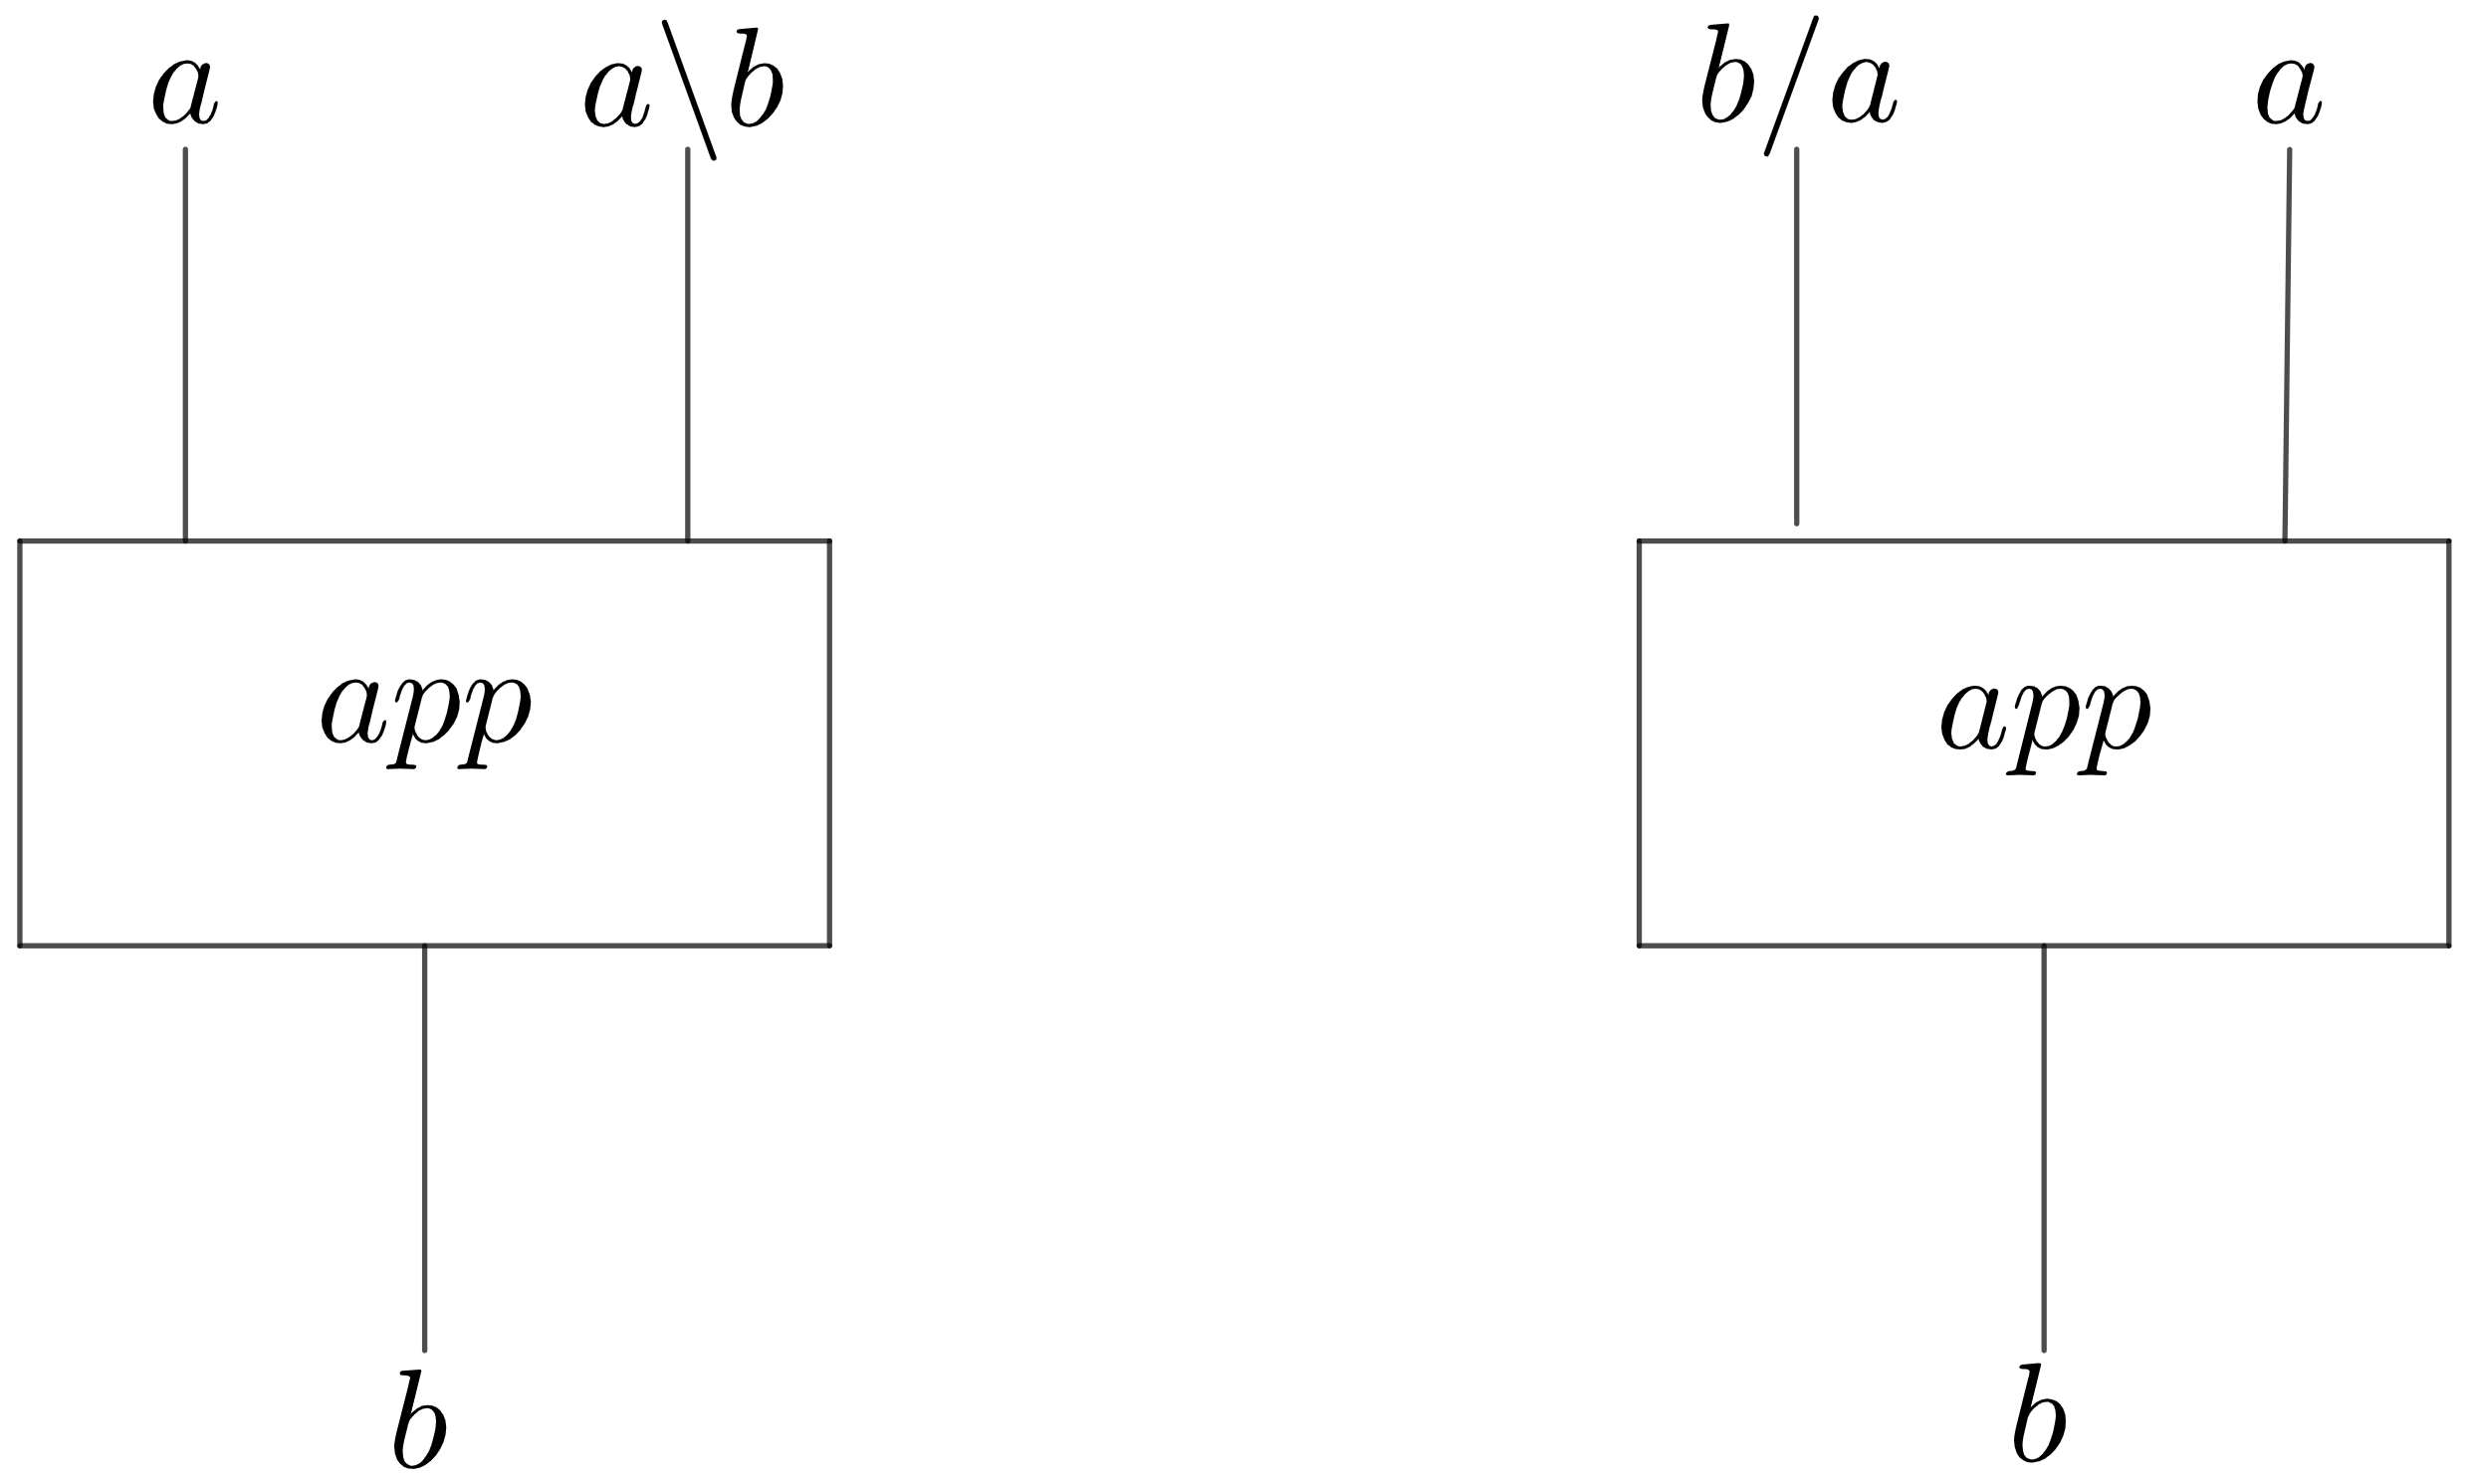
\includegraphics[scale=18]{diagrama/AB.png}
			\centering
		\end{figure}
		con $a,b \in T_{AB}(B)$. El lenguaje generado por $G$ está dado por:
		$$\mathcal{L}(G)= \{ u \in V^*|\exists g:u \to s \in \textbf{MC}(\Delta + R_{AB}) \}$$
	\end{dfn}
	
	Veamos el siguiente ejemplo:
	
	\begin{ej}
        \label{gramAB}
		Consideremos el vocabulario $V= \{ Octavio, envi\acute{o} , una, carta, a, su, amada \}$ y los tipos básicos $B= \{s,n\}$ que corresponde a una oración y a un sustantivo respectivamente. Tomemos el léxico $\Delta$ como
		$$\Delta(Octavio)=n \quad \Delta(envi\acute{o})=n \backslash (s/n) \quad \Delta(una)=n/n \quad \Delta(carta)=n$$
        $$\Delta(a)=(s\backslash s)/n \quad \Delta(su)=n/n \quad \Delta(amada)=n$$
		Entonces la oración ''Octavio envió una carta a su amada'' es gramaticalmente correcta de acuerdo a la siguiente derivación
		\begin{figure}[H]		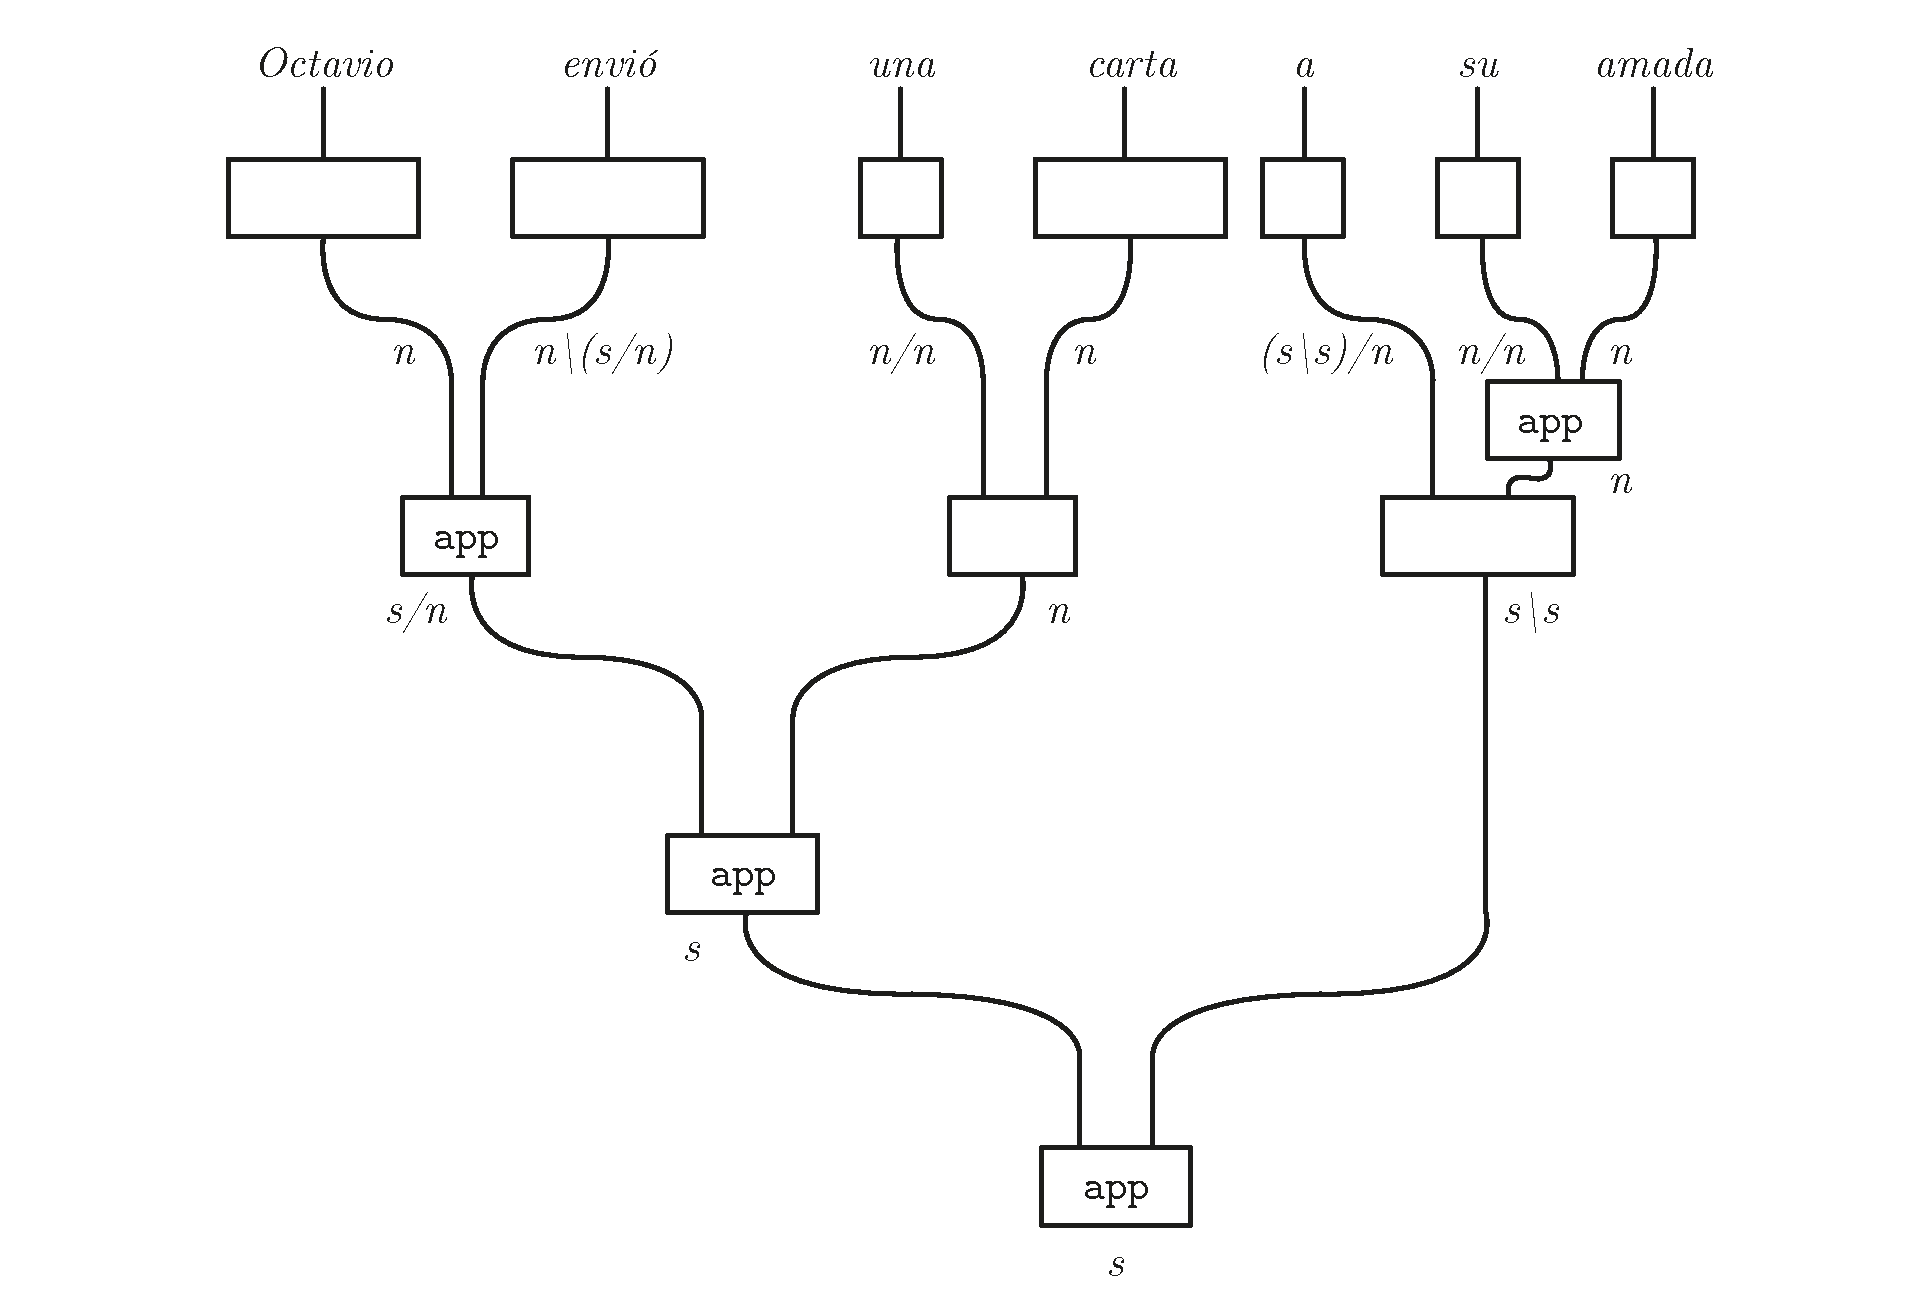
\includegraphics[scale=.45]{TeX/diagrama/4-2.pdf}
			\centering
		\end{figure}
	\end{ej}
	 
	Veamos el resultado principal de esta sección
	
	\begin{prop}
		Las gramáticas $AB$ se reducen funtorialmente a una gramática bicerrada.
	\end{prop}
	\begin{proof}
		Ya que ambas son categorías monoidales libres, para exhibir un funtor basta de las gramáticas $AB$ a las bicerradas, basta asignar a los generadores $R_[AB]$ en la bicerrada, pero veamos que estos se pueden obtener de la definición de categoría bicerrada. Sean $a,b,c$ objetos, entonces
		\begin{multicols}{2}
			\begin{prooftree}
				\hypo{a\backslash b}
				\infer1[\tt{id}]{a\backslash b \to a\backslash b}
				\infer1[\ref{curry}]{a \otimes (a \backslash b) \to b}
			\end{prooftree}
            
			\begin{prooftree}
				\hypo{a/b}
				\infer1[\tt{id}]{a/b \to a/b}
				\infer1[\ref{curry}]{(a/b)\otimes b \to a}
			\end{prooftree}
		\end{multicols}
		como queríamos probar. 
	\end{proof}
	  
	\section{Gramáticas de Lambek} 
	
	Un par de años más tarde, Joachim Lambek introdujo dos reglas más a las gramáticas categoriales: la composición y el \textit{type raising}. Aunque ambas reglas no le agregan poder expresivo a las gramáticas, sí permiten realizar las derivaciones de una manera más literal. 
	
	\begin{dfn}
		Un \textbf{gramática de Lambek} es una tupa $G=(V,B, \Delta, s)$ donde $V$ es un vocabulario, $B$ es un conjunto finito de tipos básicos y $\Delta \subset V \times T(B)$ es un léxico con la siguiente signatura $R_L$
		
		\begin{figure}[H]
			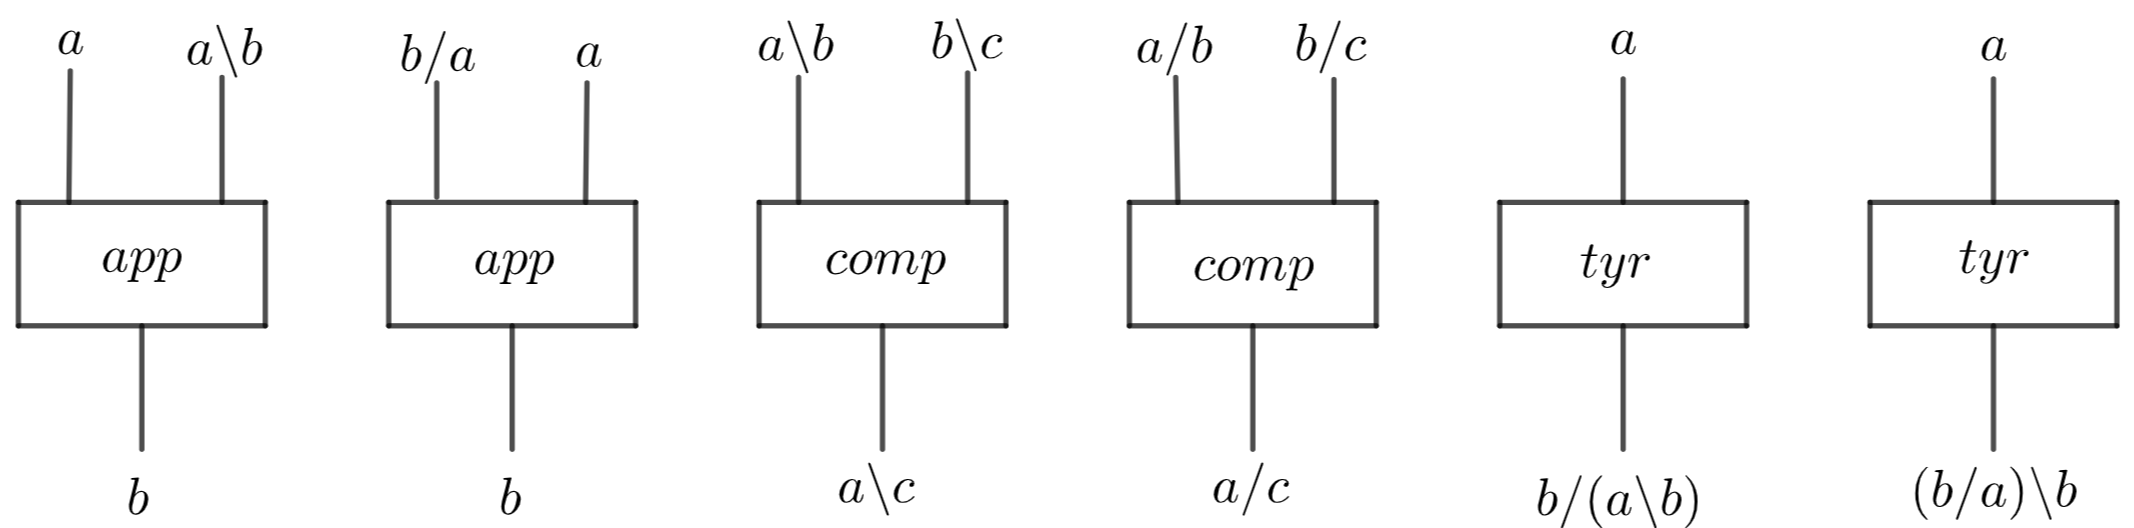
\includegraphics[scale=18]{diagrama/lambek.png}
			\centering
		\end{figure}
		El lenguaje generado por $G$ se define como
		
		$$\mathcal{L}(G)= \{ u \in V^*|\exists g:u \to s \in \textbf{MC}(\Delta + R_{L}) \}$$
		
	\end{dfn}
	
	\begin{ej}
        Consideremos el siguiente léxico
		$$\Delta(Octavio)=n \quad \Delta(enviado)=(n \backslash s)/s \quad \Delta(hab\acute{i}a)=(n \backslash s) / (n \backslash s) $$
        $$\Delta(y)=((s/n)/(s/n))/(s/n) \quad \Delta(Eliza)=n$$
        $$\Delta(respondi\acute{o})=(n\backslash s)/n \quad \Delta(la)=n/n \quad \Delta(carta)=n$$
        Entonces tenemos la siguiente derivación de la oración ''Octavio había enviado y Eliza recibió una carta''
        \begin{figure}[H]		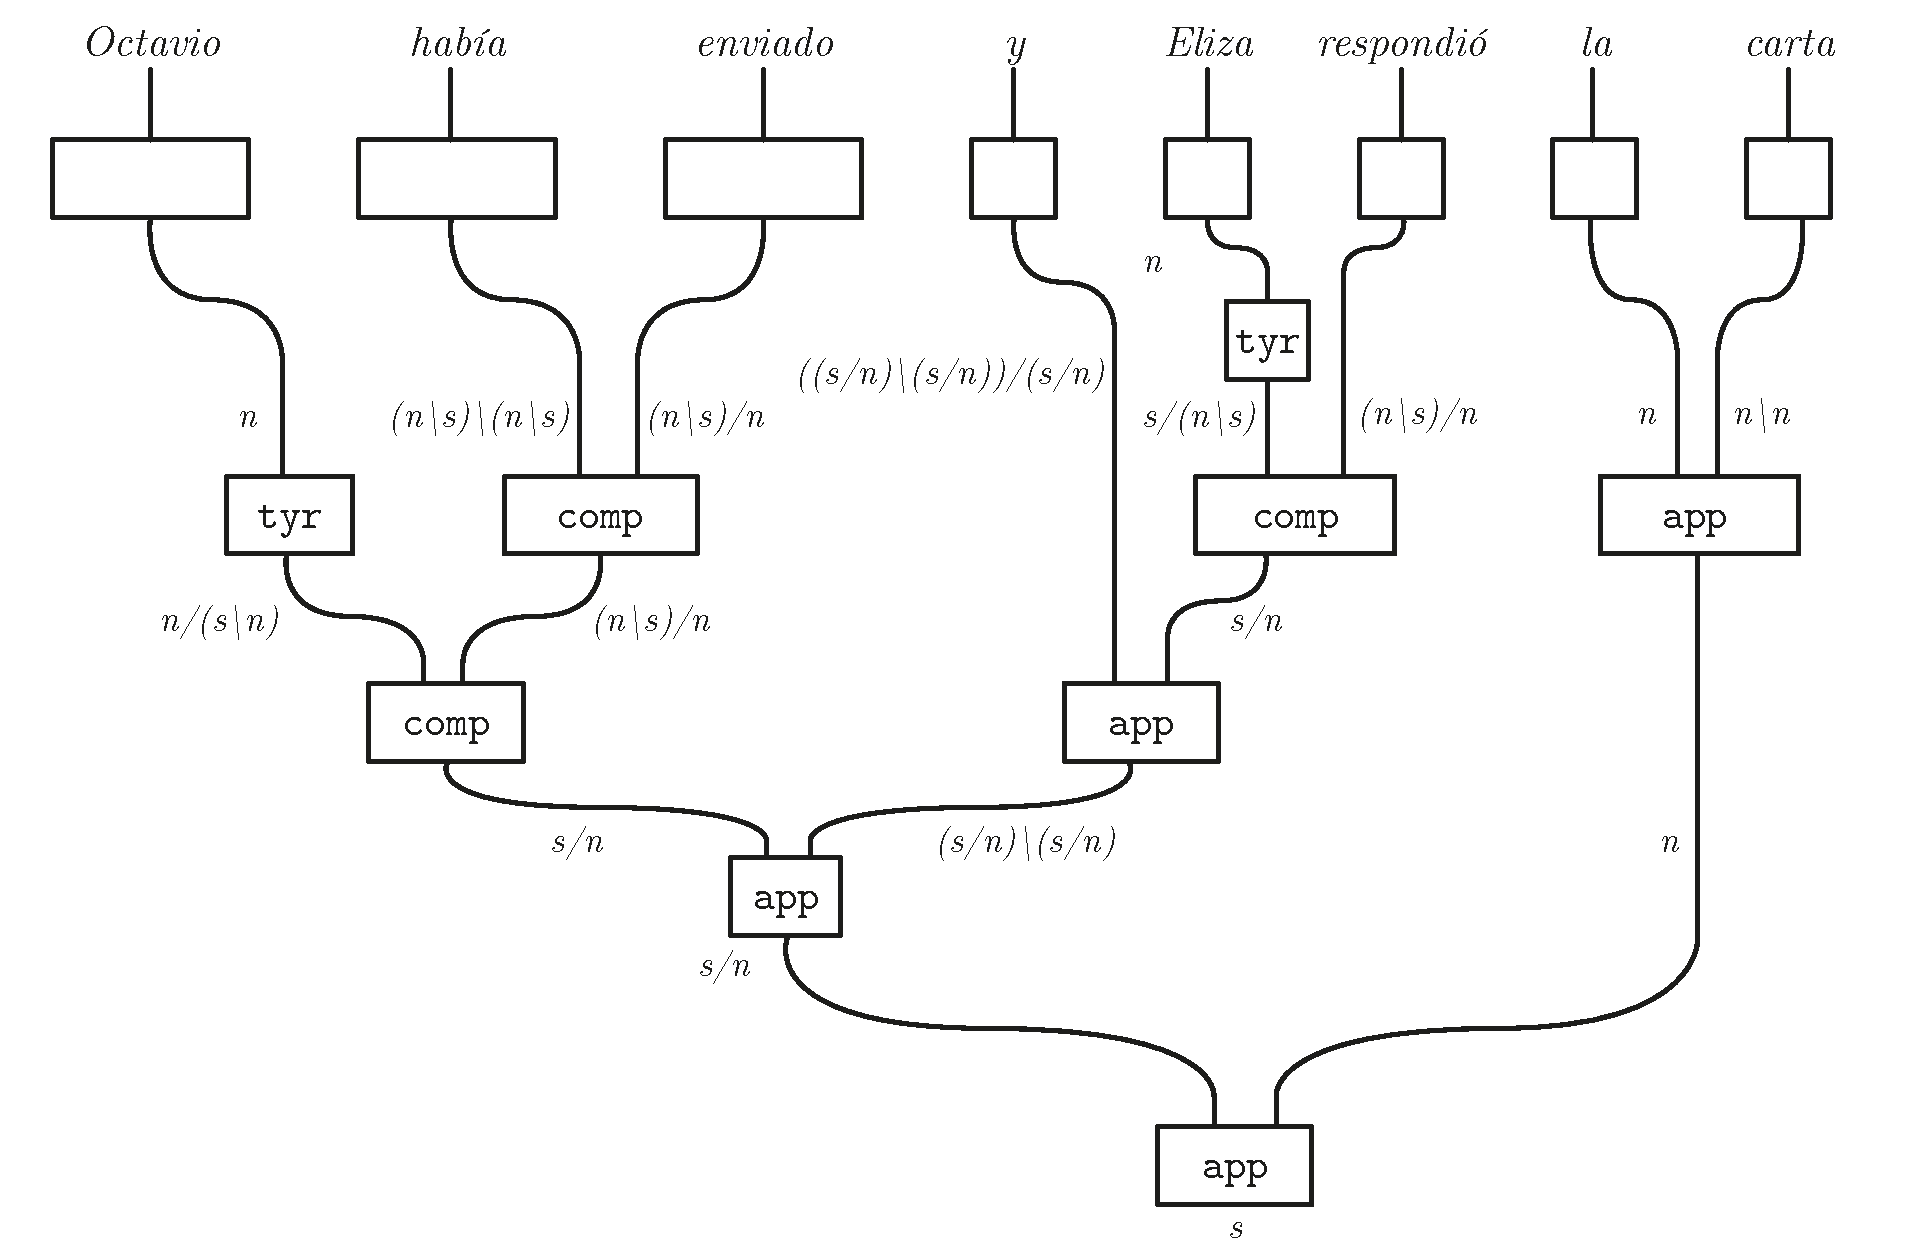
\includegraphics[scale=.45]{TeX/diagrama/4-3.pdf}
			\centering
		\end{figure}
	\end{ej}
	
	\begin{prop}
		Las gramáticas $AB$ se reducen funtorialmente a una gramática bicerrada.
	\end{prop} 
	\begin{proof}
		Como en la proposición anterior, basta ver que podemos generar $R_L$ en una categoría bicerrada. Ya sabemos que las dos $app$ son posibles, veamos el resto. Sean $a,b$ objetos. Construyamos las derivaciones correspondientes a $comp$.
		\begin{multicols}{2}
			\begin{center}
			\begin{prooftree}
				\hypo{a \backslash c}
				\infer1[{\tt{id}}]{a \backslash c \to a \backslash c}
				\infer1[\ref{curry}]{a \otimes a \backslash b \to b}
				\hypo{b \backslash c}
				\infer1[{\tt{id}}]{b \backslash c \to b \backslash c}
				\infer2[$\otimes$ \text{ y } $\circ$]{a \otimes a \backslash b \otimes b \backslash c \to c}
				\infer1[\ref{curry}]{a \backslash b \otimes b \backslash c \to a \backslash c}
			\end{prooftree}
            \end{center}
            \begin{center}
			\begin{prooftree}
				\hypo{a/b}
				\infer1[\tt{id}]{a/b \to a/b}
				\hypo{b/c}
				\infer1[\tt{id}]{b/c \to b/c}
				\infer1[\ref{curry}]{b/c \otimes c \to b}
				\infer2[$\otimes$ \text{ y } $\circ$]{a/b \otimes b/c \otimes c \to a}
				\infer1[\ref{curry}]{a/b \otimes b/c \to a/c}
			\end{prooftree}
            \end{center}
		\end{multicols}
		Concluyamos con las derivaciones de $tyr$.
		\begin{multicols}{2}
            \begin{center}
			\begin{prooftree}
				\hypo{a \backslash b}
				\infer1[{\tt{id}}]{a \backslash b \to a \backslash b}
				\infer1[\ref{curry}]{a \otimes (a \backslash b) \to b}
				\infer1[\ref{curry}]{a \to b/(a \backslash b)}
			\end{prooftree}
            \end{center}
            \begin{center}
			\begin{prooftree}
				\hypo{b/a}
				\infer1[{\tt{id}}]{b/a \to b/a}
				\infer1[\ref{curry}]{(b/a)\otimes a \to b}
				\infer1[\ref{curry}]{a \to (b/a) \backslash b}
			\end{prooftree}
            \end{center}
		\end{multicols} 
		con lo cual terminamos la prueba. 
	\end{proof}
	
	\section{Gramáticas combinatoria}
	
	En los ochentas, Stuart Schieber demostró que hay lenguas que no pueden ser generadas por gramáticas libres de contexto, esto es porque ciertas oraciones involucran de manera natural dependencias cruzadas, fenómeno que ocurre cuando dos series de palabras se mezclan entre sí. Aunque el fenómeno no es usual en español o inglés, es muy común en el suizo-alemán. Veamos el siguiente ejemplo.
    \begin{center}
        \textit{''... mer \textcolor{red}{em Hans} \textcolor{blue}{es huss} \textcolor{red}{halfed} \textcolor{blue}{aastriiche}''} \\   
    \end{center}
	que se traduce como ''... nosotros \textcolor{red}{ayudamos a Hans} a \textcolor{blue}{pintar la casa}''.\\
    \setulcolor{red}
	Ejemplos sencillos en el español son las oraciones ''\textcolor{blue}{Ayer}  \textcolor{blue}{\ul{una mujer} llegó} \ul{que conocía}'' y ''Octavio envió a su amada una carta''.
	Para analizar estos casos, se extienden las gramáticas anteriores a la gramática categorial combinatoria mediante la inclusión de dos reglas de composición cruzada.
	
	\begin{dfn}
		Una \textbf{gramática categorial combinatoria (GCC)} es una tupla $G=(V,B, \Delta, s)$ donde $V$ es un vocabulario, $B$ es un conjunto de tipos y $\Delta \subset V \times T(B)$ es un léxico. La signatura $R_{GCC}$ es la signatura $R_{L}$ más las siguientes dos reglas para todo $a,b,c$ objeto:
		\begin{figure}[H]
			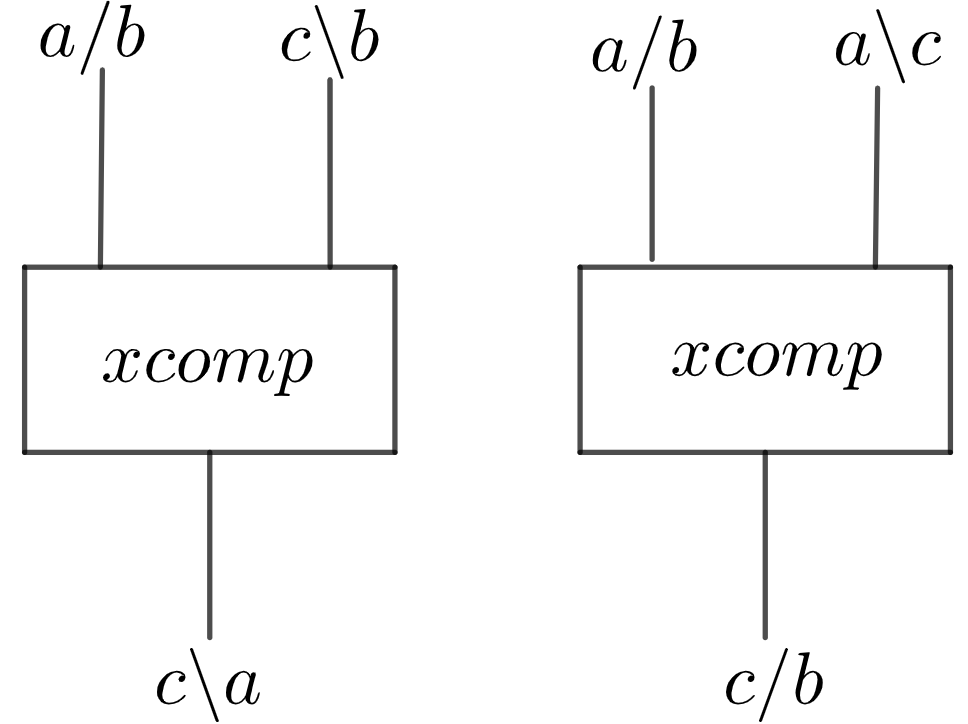
\includegraphics[scale=18]{diagrama/CCG.png}
			\centering
		\end{figure}
		El lenguaje generado por $G$ se define como
		
		$$\mathcal{L}(G)= \{ u \in V^*|\exists g:u \to s \in \textbf{MC}(\Delta + R_{GCC}) \}$$
	\end{dfn}
	\begin{ej}
		Consideremos el vocabulario del ejemplo \ref{gramAB}. Tenemos la siguiente derivación de la oración ''Octavio envió a su amada una carta''.
        \begin{figure}[H]		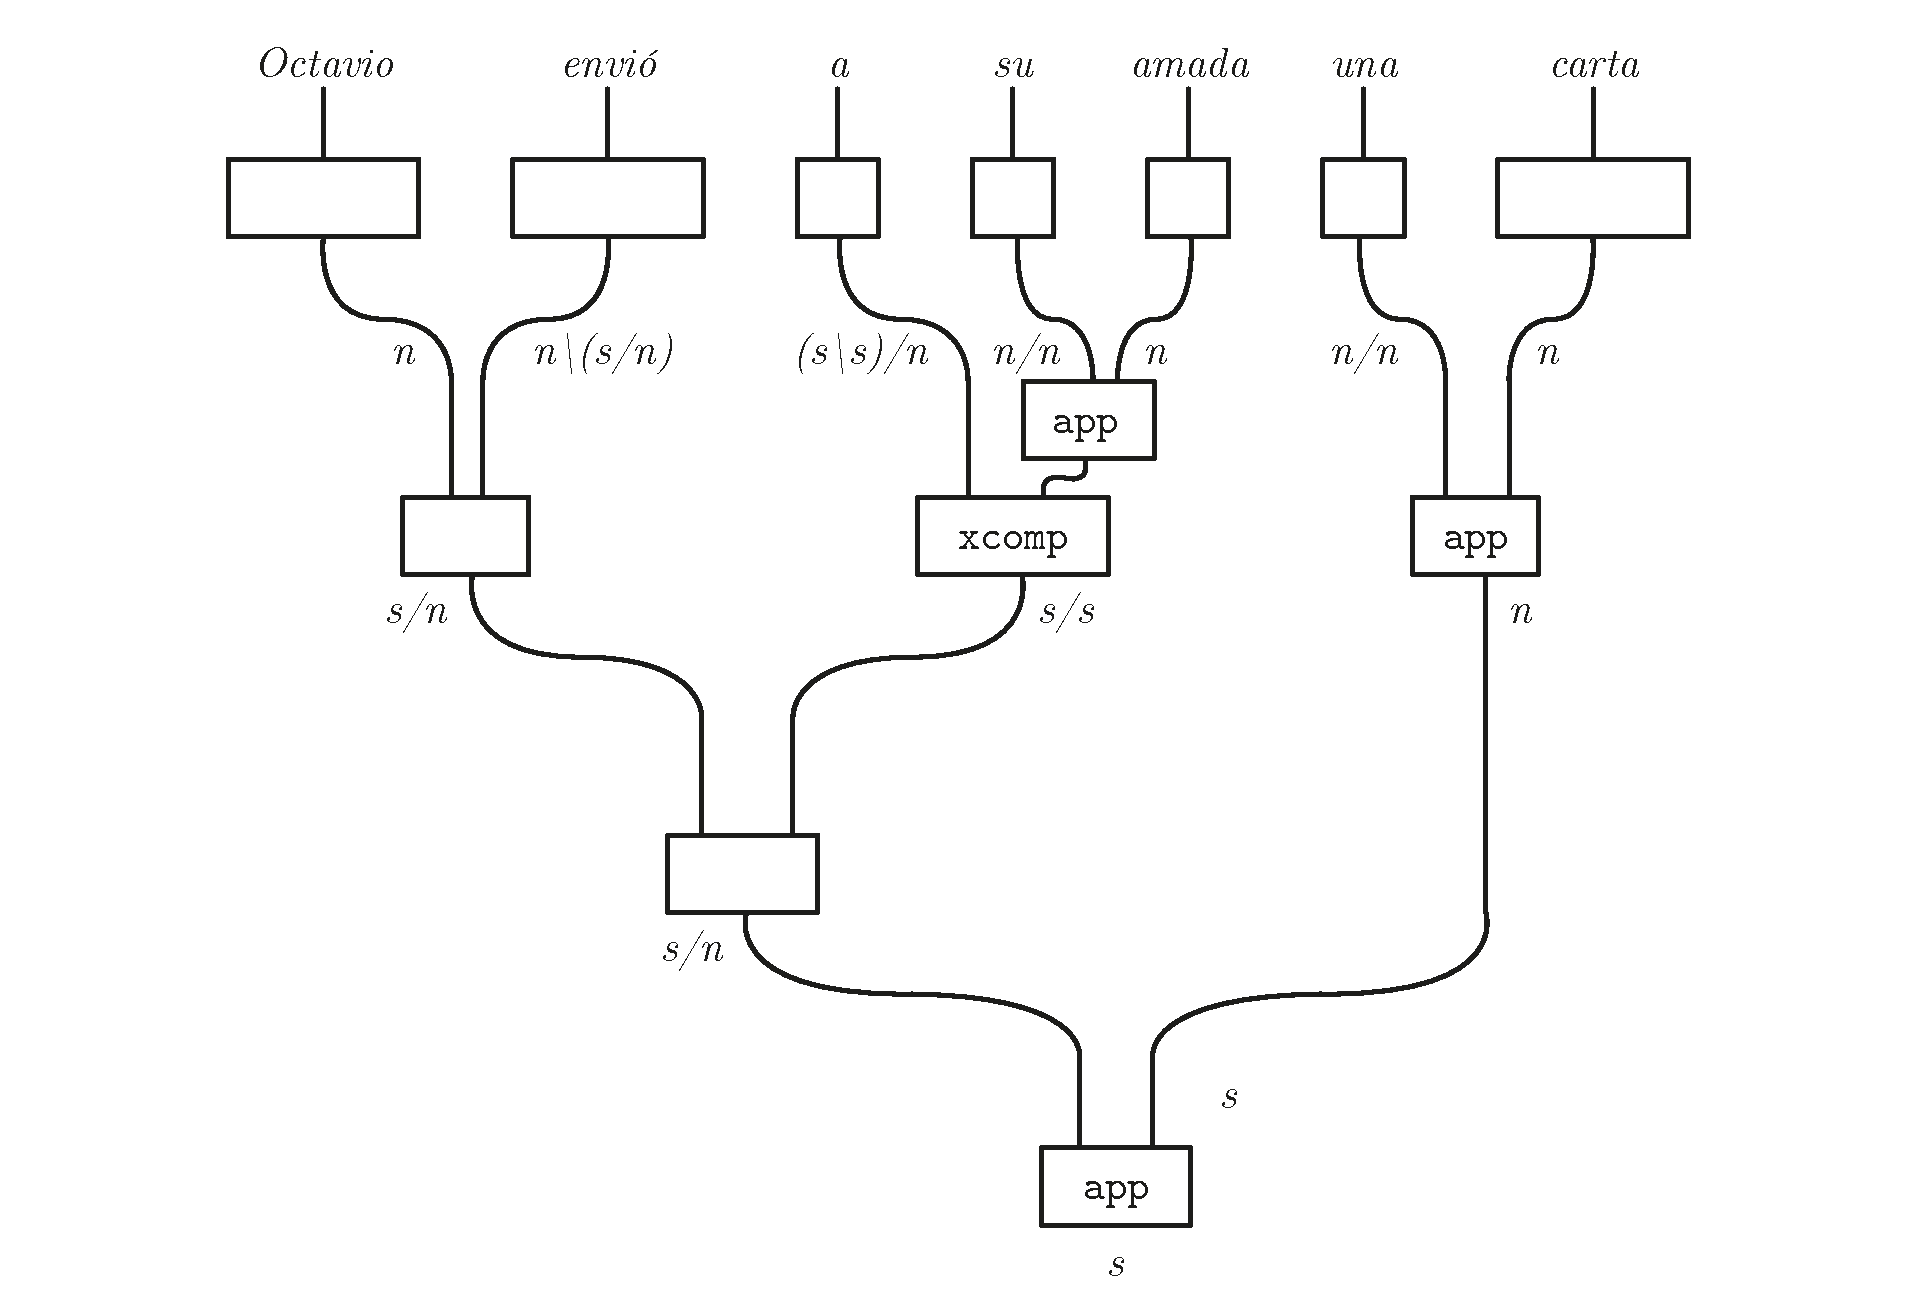
\includegraphics[scale=.45]{TeX/diagrama/4-1.pdf}
			\centering
		\end{figure}
	\end{ej}
	A diferencia de las dos gramáticas categoriales anteriores, la signatura de $CCG$ no puede ser deducida de los axiomas de categoría bicerrada, pues todos los axiomas preservan el orden de los tipos. Así, nuestro mejor intento sería agregar directamente las reglas $xcomp$ a la signatura de las gramáticas monoidales, o bien, trabajar en categorías cerradas.
	
	\begin{dfn}
		Una \textbf{categoría monoidal simétrica} $\mathcal{C}$ es una categoría monoidal junto a una transformación natural $\sigma:a\otimes b \to b \otimes a$ que satisface  
		\begin{figure}[H]
			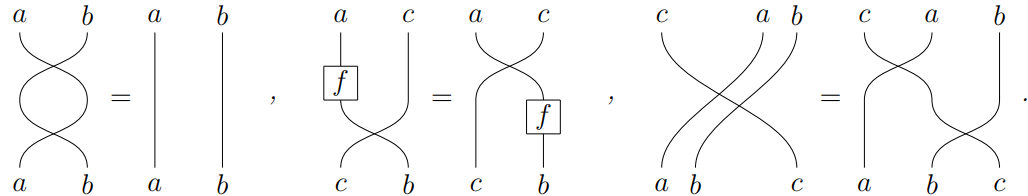
\includegraphics[scale=.5]{diagrama/swap.png}
			\centering
		\end{figure}
		para cualesquiera $a,b,c \in \mathcal{C}_0$ y $f:a \to b \in \mathcal{C}_1$.
	\end{dfn} 
	
	\begin{dfn}
		Una categoría cerrada es una categoría simétrica bicerrada.
	\end{dfn}
	
	\begin{prop}
		Una categoría cerrada tiene las reglas $xcomp$ como morfismos.
	\end{prop}
	\begin{proof}
		Sean $a,b,c$ objetos una categoría cerrada libre. Basta mostrar las derivaciones para $xcomp$.
		\begin{multicols}{2}
		\begin{prooftree}
			\hypo{a/b}
			\infer1[{\tt{id}}]{a/b \to a/b}
			\hypo{c \backslash b}
			\infer1[{\tt{id}}]{c \backslash b \to c \backslash b}
			\infer1[\ref{curry}]{c \otimes c \backslash b \to b}
			\infer2[$\otimes$ y $\circ$]{a/b \otimes c \otimes c \backslash b \to a}
			\infer1[$\sigma$]{c\otimes a/b \otimes c \backslash b \to a}
			\infer1[\ref{curry}]{a/b \otimes c \backslash b \to c \backslash a}
		\end{prooftree}
			\begin{prooftree}
				\hypo{a/b}
				\infer1[{\tt{id}}]{a/b \to a/b}
				\infer1[\ref{curry}]{a/b \otimes b \to a}
				\hypo{a \backslash c}
				\infer1[{\tt{id}}]{a \backslash c \to a \backslash c}
				\infer2[$\otimes$ y $\circ$]{a/b \otimes b \otimes a \backslash c \to c}
				\infer1[$\sigma$]{a/b \otimes a \backslash c \otimes b \to c}
				\infer1[\ref{curry}]{a/b \otimes a \backslash c \to c/b}
			\end{prooftree}
		\end{multicols}
		
	\end{proof}
	
	Una última observación es que podría resultar una mala idea trabajar gramáticas sobre categorías cerradas sin restricciones, pues entonces corremos el riesgo de perder el orden de las palabras en una oración, por lo cual restringimos los morfismos $f:u \to s$ a la aplicación exclusiva de $\textit{xcomp}$. \\
	
\end{document}